\section{Riverflow \dcsecondauthorshort} 
\label{sec:fahrspurerkennung:riverflow}

Der dritte und final genutzte Ansatz zur Fahrspurerkennung nutzt im Gegensatz zu den vorherigen Varianten kein durch wenige Parameter (Polynomkoeffizienten etc.) beschreibbares Modell. Dem Objekt Fahrspur werden hingegen bestimmte Eigenschaften zugesprochen, welche zur Idee des Riverflow-Algorithmus \autocite{limRiverFlowLane2012} und der angeschlossenen Punkteverifikation geführt haben.
\begin{enumerate}
\item \label{item:riverflow:rule:solidline}
Ist eine Fahrbahnmarkierung eine Randlinie, so ist dies eine nicht unterbrochene Markierung bestimmter Breite.
\item \label{item:riverflow:rule:dashedline}
Ist eine Fahrbahnmarkierung eine Mittellinie, so besteht diese aus Elementen deren Länge, Breite und Abstand voneinander konstant und bekannt sind.
\item \label{item:riverflow:rule:curvature}
Die Krümmung einer Fahrbahnmarkierung darf einen bestimmten Wert nicht überschreiten.
\item \label{item:riverflow:rule:distance}
Rechte-, Mittel- und Seitenlinie besitzen einen konstanten Abstand (Fahrspurbreite) zueinander.
\end{enumerate}
\subsection{Mittellinie}
\label{ssec:fahrspurerkennung:riverflow:mittellinie}
Ähnlich wie im Kapitel~\ref{sec:maskenbau} beschrieben findet dieser Ansatz die zur Mittellinie zugehörigen Elemente, ohne auf richtig definierte \gls{acr:roi} angewiesen zu sein. Ausgangspunkt ist ebenfalls wieder das binarisierte Bild, auf das die \gls{glos:matlab}-Funktion \emph{regionprops} angewendet wird. Diese bereits verfügbare Funktion findet als Alternative zum in ~\ref{sec:maskenbau} erwähnten \glqq Ringfilter\grqq{} alle zusammenhängende Pixelgruppen und extrahiert zusätzlich eine Vielzahl derer Eigenschaften, wie Länge, Breite, Orientierung und Mittelpunkt. Da wie in Punkt~\ref{item:riverflow:rule:dashedline} bereits erwähnt die mittlere Fahrbahnmarkierung genau spezifiziert ist, werden so alle potentiellen Mittellinienstriche vorgemerkt. Diese Vorgehensweise funktioniert allerdings nur dann stabil, wenn die Güte des binarisierten Bildes gut genug ist, sodass Striche \gls{acr:zb} nicht unterbrochen sind. Trotz der guten Qualität des Bildes kommt es vor, dass falsche Bildteile als Mittellinienelemente erkannt und vorgemerkt werden. Deswegen stellen wir durch eine Verifizierung sicher, dass möglichst keine falschen Punkte in die Weltkarte, welche später zur Regelung des Autos genutzt wird, eingetragen werden. Schon an der großen Vier-Seiten-Kreuzung kommt es sonst zum Problem, dass darüber hinaus Mittellinienstriche der kreuzenden Straße erkannt werden. Auch wenn diese zur mittleren Linie gehören, sollen sie hier auf Grund des derzeitigen Regelungskonzepts noch nicht in die Karte aufgenommen werden. 
% Das ist freilich nicht falsch, aber für das aktuelle Regelungskonzept auch nicht zielführend. 

\paragraph{Verifikation}

Die Prozedur der Verifizierung verläuft nach einem vergleichbaren Prinzip wie der in~\ref{ssec:fahrspurerkennung:riverflow:randlinie} beschriebene Riverflow-Algorithmus. Dabei wird davon ausgegangen, dass sich das Fahrzeug größtenteils in der Fahrspur befindet, sodass mindestens ein Mittellinienstrich unweit vor dem Auto positioniert ist. Initial wird ein Suchfenster erstellt, welches in der Höhe den reichlichen Abstand zwischen den Mittelpunkten zweier benachbarter Mittelstreifen annimmt. Das erste sich in diesem Bereich aufhaltende Objekt wird dann als verifiziert angesehen, wenn seine Orientierung nicht übermäßig von der des Fahrzeugs abweicht. Ausgehend von diesem Punkt \glqq hangelt\grqq{} sich der Verifikations-Algorithmus von Strich zu Strich, indem er eine neue \gls{acr:roi} (ein neues Suchfenster) aufstellt. Da zu jedem (verifizierten) Punkt seine Orientierung bekannt ist, wird der nächste Mittellinienpunkt in dieser Richtung im ebenfalls bekannten Abstand zwischen zwei Punkten vermutet und dort der Mittelpunkt des neuen Suchfensters definiert. Dieses Schema wiederholt sich, bis entweder der Bildrand erreicht ist, keine Punkte im Suchfenster liegen, oder sich die Orientierung von einem zum nächsten Strich zu stark geändert hat.

Das gleiche Vorgehen wird zudem wahlweise vom ersten Punkt hinter dem Fahrzeug ausgehend wiederholt, sodass auch schon passierte Mittellinienpunkte, welche \gls{acr:zb} bei einem zukünftigen Überholvorgang benötigt werden könnten, verifiziert sind.

\begin{figure}[H]
	\centering
	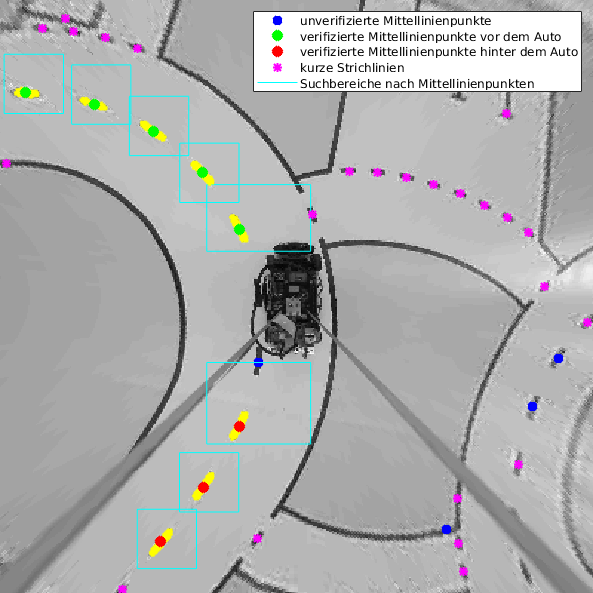
\includegraphics[width=0.9\textwidth]{fahrspurerkennung_riverflow_regionprops.png}
	\caption{Detektion von Punktgruppen mit bestimmten Eigenschaften mithilfe der \emph{regionprops}-Funktion}
	\label{fig:riverflow:mittellinie:regionprops}
\end{figure}

In \gls{acr:abb}~\ref{fig:riverflow:mittellinie:regionprops} sehen wir das Resultat der Mittellinien-/Stricherkennung. Im gleichen Zug wird die \emph{regionprops}-Funktion auch zur Randstricherkennung bei Kreuzungen genutzt. Diese Informationen werden im Riverflow-Algorithmus verwendet, welcher im nun folgenden Abschnitt beschrieben ist.
\subsection{Randlinie}
\subsubsection{Startpunktgewinnung}
Um den eigentlichen Riverflow-Algorithmus ausführen zu können werden wird die ungefähre Lage der seitlichen Fahrbahnmarkierungen in der Nähe des Fahrzeugs benötigt. Zur Ermittlung dieser gibt es 3 Möglichkeiten:
\begin{enumerate}
\item \label{item:solidline:startpoints:dashedline}
Die Bestimmung durch Orientierung und Position des ersten vor dem Fahzeug gelegenen Mittellinienelementes. Hierzu wird der Mittelpunkt des Elementes entlang der Orientierung desselbigen um die Fahrspurbreite nach links/rechts verschoben. BILD
\item \label{item:solidline:startpoints:hough}
Eine eindimensionale Hough-Transformation des Bildausschnittes direkt vor dem Fahrzeug wie in REFERENZ beschrieben. BILD
\item \label{item:solidline:startpoints:fixed}
Annahme einer festen Position vor dem Fahrzeug/im Kamerabild.
\end{enumerate}

\subsubsection{zentraler Algorithmus}
Durch Nutzung der Eigenschaften \ref{item:riverflow:rule:solidline} und  \ref{item:riverflow:rule:curvature} kann ausgehend von der aktuellen Linienorientierung in einem bestimmten Kegel, dessen Öffnungswinkel durch die maximale Krümmung der Fahrspur definiert ist, der weitere Verlauf der Fahrbahnmarkierung vermutet werden. BILD
Algorithmisch genutzt wird dieses Wissen durch die Verwendung der aus \ref{ssec:fahrspurerkennung:kalman:messung} bekannten \glspl{glos:scanline}.
Zuerst wird ein Verschiebungsvektor \begin{math} \boldsymbol{v_n} \end{math} zwischen vorletztem (\begin{math} \boldsymbol{p_{n-1}} \end{math}) und letztem gefundenen Punkt  (\begin{math} \boldsymbol{p_n} \end{math})  der Fahrbahnmarkierung gebildet \eqref{eq:riverflow:solidline:dispvec}. Ausgehend vom letzten gefundenen Punkt der Linie (\begin{math} \boldsymbol{p_n} \end{math}) wird selbiger nun um den Vektor \begin{math} \boldsymbol{v_n} \end{math} weiterverschoben und bildet den Mittelpunkt  \begin{math} \boldsymbol{m_{n+1}}  \end{math} der nächsten \gls{glos:scanline} \eqref{eq:riverflow:solidline:scanlinemidpoint}.
\begin{equation}
\label{eq:riverflow:solidline:dispvec}
\boldsymbol{v_n} =  \boldsymbol{p_n} - \boldsymbol{p_{n-1}}
\end{equation}
\begin{equation}
\label{eq:riverflow:solidline:scanlinemidpoint}
\boldsymbol{m_{n+1}} =  \boldsymbol{p_n} + \boldsymbol{v_n}
\end{equation}
 Die \gls{glos:scanline} kann nun durch senkrecht zum Verschiebungsvektor \begin{math} \boldsymbol{v_n} \end{math}  durch den Punkt \(\boldsymbol{m_{n+1}}\) konstruiert werden.
Da die Filterantwort des Kantendetekors durch den Algorithmus zur Erkennung der Mittellinie schon für das gesamte Bild vorliegt, kann direkt nach Maxima unter den Pixeln, welche die \gls{glos:scanline} schneidet, gesucht werden

\subsubsection{Sonderfall gestrichelte Randlinien}
\subsubsection{Ende}
\subsection{Verifikation der seitlichen Fahrbahnmarkierungen \dcsecondauthorshort}
\label{ssec:fahrspurerkennung:riverflow:verifikation}
Nachdem für Mittel- und Seitenlinie repräsentative Punkte aus dem Bild extrahiert wurden, gilt es deren Sinnhaftigkeit zu überprüfen. Somit können:
\begin{enumerate}
\item Falsch erkannte Fahrbahnmarkierungen eliminiert werden.
\item Bei Vorhandensein mehrerer Hypothesen für die Seitenlinien die Besten ausgewählt werden.
\end{enumerate}

\subsubsection{Seitenlinienvergleich} 
\label{sssec:fahrspurerkennung:riverflow:verifikation:seitenlinienvergleich}
Zuerst wiFensters

\begin{figure}[htbp] % [htb]rd der Abstand der äußeren Fahrbahnmarkierungen zueinander geprüft. Diese Validierung bedient sich ineinander verschachtelter Schleifen, um zu jedem Punkt das passende Gegenüber zu finden. Exemplarisch wird diese Schachtelung nun am Beispiel der Beurteilung der linken Fahrbahnmarkierungspunkte anhand der rechten Linie dargelegt. Es wird:
\begin{enumerate}
\item 
Eine Hypothese der linken Linie gewählt.
\item \label{item:riverflow:verification:l_r:loops:right_hypo}
Eine Hypothese der rechten Fahrbahnmarkierung selektiert.
\item \label{item:riverflow:verification:l_r:loops:point}
Ein Punkt der gewählten linken Linienhypothese ausgesucht.
\end{enumerate}
Nun kann simultan der Abstand \nrm{\gls{lat:av}} \eqref{eq:norm:distpoints} 
zu allen Punkten der gewählten rechten Fahrbahnmarkierungshypothese berechnet werden. 
\begin{equation}
\label{eq:norm:distpoints} 
\nrm{\gls{lat:av}} = \nrm{\pnt{p_{\text{links}}} - \pnt{p_{\text{rechts}}}} 
\end{equation}
Da der nächstgelegene Punkt der rechten Linienhypothese zum gewählten Punkt der linken Fahrbahnmarkierungshypothese gefragt ist, wird nur das kleinste Ergebnis dieser simultanen Berechnung weiter betrachtet.

Die Koordinatenserie der linken Linienhypothese wird vom Anfgangspunkt des Riverflow-Algorithmus bis
\begin{itemize}
\item der Endpunkt derselben erreicht ist 
\item der Abstand zur gewählten rechten Fahrbahnmarkierungshypothese einmal überschritten wurde
\end{itemize}
nacheinander bearbeitet (siehe Schleife~\ref{item:riverflow:verification:l_r:loops:point}). Die so anhand einer selektierten rechten Linienhypothese verifizierte linke Koordinatenserie wird zwischengespeichert. 
Nach Validieren mittels aller rechten Fahrbahnmarkierungshypothesen (siehe Schleife~\ref{item:riverflow:verification:l_r:loops:right_hypo}) kann nun die längste verifizierte Koordinatenserie der gewählten linken Linienhypothese ermittelt werden.

Der beschriebene Prozess wird nun für alle linken Fahrbahnmarkierungshypothesen ausgeführt. Die linke Linienhypothese mit der größten Anzahl Punkte wird als mithilfe der rechten Fahrbahnmarkierung validierte linke Linie betrachtet. Der prinzipiell gleiche Algorithmus wird für die Verifikation der rechten Fahrbahnmarkierung anhand der linken Linie genutzt.

\subsubsection{Beurteilung der Seitenlinien anhand der mittleren Fahrbahnmarkierung}
\paragraph{lineare Interpolation}
Da in einem Bild signifikant weniger Mittellinienpunkte (genauer: Mittelpunkte der Mittellinienelemente) als Punkte der seitlichen Fahrbahnmarkierung gefunden werden, müssen zur Validierung der Seitenlinienpunkte durch die mittlere Fahrbahnmarkierung zusätzliche Punkte auf selbiger erzeugt werden. Hierfür wird jeweils der Mittelpunkt der Gerade zwischen zwei Mittellinienpunkten genutzt. Bei \( n \) Mittellinienpunkten entstehen also \( n-1 \) linear interpolierte Punkte.
\begin{equation}
\pnt{p_{\text{interpoliert}i}} = (\pnt{p_{\text{real}i}}+\pnt{p_{\text{real}i+1}})/2 
\end{equation}
\paragraph{Algorithmus} Die Prozedur zum Vergleich der Seitenlinien mit der mittleren Fahrbahnmarkierung ist weitgehend identisch mit Abschnitt~\ref{sssec:fahrspurerkennung:riverflow:verifikation:seitenlinienvergleich}. Lediglich das Auswählen einer Hypothese der Mittellinie entfällt, da hier in jedem Fall nur ein möglicher Verlauf gefunden wird.

\subsubsection{Zusammenführung der Verifikationsmethoden}
Lieferte die Überprüfung der seitlichen Fahrbahnmarkierungen aneinander die längere Koordinatenserie, so wird diese weiter verwendet. Andernfalls wird die Menge der an der mittleren Linie validierten Punkte genutzt.